% CS 455, SP'24 Software Requirements Document template
% Software requirements template based on the template from
% https://tex.stackexchange.com/questions/42602/software-requirements-specification-with-latex
%
\documentclass[letterpaper,12pt,oneside,listof=totoc]{scrreprt}
\usepackage{listings}
\usepackage{underscore}
\usepackage[bookmarks=true]{hyperref}
\usepackage{xurl}
\usepackage{graphicx}
\usepackage{float}

\hypersetup{
    % bookmarks=false,                                % show bookmarks bar
    pdftitle={Software Requirements Specification}, % title
%    pdfauthor={Yiannis Lazarides},                  % author
%    pdfsubject={TeX and LaTeX},                     % subject of the document
%    pdfkeywords={TeX, LaTeX, graphics, images},     % list of keywords
    colorlinks=true,                                % false: boxed links; true: colored links
    linkcolor=blue,                                 % color of internal links
    citecolor=black,                                % color of links to bibliography
    filecolor=black,                                % color of file links
    urlcolor=black,                                % color of external links
    linktoc=page                                    % only page is linked
}%
\def\myversion{0.2}

\date{\today}
\author{} % suppress warning, do not fill this in
\begin{document}

% we don't use \maketitle because we overide the default title page here
\begin{titlepage}
\flushright
\rule{\textwidth}{5pt}\vskip1cm
\Huge{SOFTWARE REQUIREMENTS SPECIFICATION}\\
\vspace{1.5cm}
for\\
\vspace{1.5cm}
Software Risk Tracking\\                      %%% Update the title page text
\vspace{1.5cm}
\LARGE{Release 0.2\\}
\vspace{1.5cm}
%\LARGE{Version \myversion approved\\}
\vspace{1.5cm}
Prepared by Software Risk Tracking Team\\
\vfill
\rule{\textwidth}{5pt}
\end{titlepage}

\tableofcontents
% this will be automatically created from chapters, sections, and subsections

\listoffigures
% this will be automatically created from the figure environment

\newpage

\listoftables
% this will be automatically created from the table environment

\chapter*{Revision History}
% Update this table for each approved/baselined revision of the requirements
% Add the new content followed by a \hline

\begin{tabular}{| c | p{0.30\textwidth} | p{0.50\textwidth} |}
\hline
Date     & Description   & Revised by \\
\hline
2/21/24 & Baseline & Software Risk Tracking Team \\
\hline
3/2/24 & Version 0.2 & Software Risk Tracking Team \\
\hline
\end{tabular}


\chapter{INTRODUCTION}

\section{Purpose}
% purpose of this document
   The purpose of this document is to build a software risk-tracking system that will identify risks and help the business streamline its Software. It will keep track of the impact of risk and its status. Once completed it will help the team analyze the risks according to their ranks and solve accordingly.                 \setlength{\parskip}{0em}
\section{Document Conventions}
    This SRS document conforms to the IEEE Standards Style Manual, ensuring consistency and clarity in the communication of requirements. The term "shall" is used to indicate mandatory requirements which must be strictly followed. The term "should" suggests a course of action among several possibilities, recommended for its suitability, though not exclusively mandated. "May" indicates a permissible course of action within the requirements' limits. The phrases "must" and "will" are deprecated for describing mandatory requirements in this document. For data entry fields, "text" or "printable text" refers to any printable alphanumeric character available on the US standard keyboard, excluding tabs, carriage returns, new lines, and other non-printable or control characters. When "numeric" is indicated for a data entry field, only digits are permitted, and characters such as dashes, commas, or periods are excluded unless specifically allowed.
    \setlength{\parskip}{0em}
% how to read this document
% for example "conforms to IEEE Standards Style Manual"
% which defines "shall" "should" "may" and typographic conventions

\section{Acronyms} 

% add a table here for acronyms
\begin{table} [H]
\begin{center}
\begin{tabular}{|c|c|}
    \hline
    CS  &  Computer Science \\
    \hline
    BSD & Berkeley Software Distribution \\
    \hline
    OS  & Operating System \\
    \hline
    AMD & Advanced Micro Devices \\
    \hline
    STL & Standard Template Library \\
    \hline
    SQL & Structured Query Language \\
    \hline
    GB  & Giga Byte \\
    \hline
    RAM & Random Access Memory \\
    \hline
    RMS & Risk Management System\\
    \hline
    ERP & Enterprise Resource Planning \\
    \hline
    CRM & Customer Relationship Management \\
    \hline
    REST & Representational State Transfer \\ 
    \hline
    API & Application Programming Interface \\
    \hline
    IEEE & the Institute of Electrical and Electronics Engineers \\
    \hline
\end{tabular}
\end{center}
\caption{Acronym List}
\end{table}
% list of acronyms used in this document
% that the typical reader won't know

\section{Project Scope and Product Features}
% high level description of what is in scope and what is
% out of scope for the software
The purpose of the risk tracking system is to help maintain a tracked list of risks to aid in the management of said risks. \newline

\noindent The application allows admin users to perform the following tasks: add/edit/delete users, assign a single or multiple roles to users, create and maintain risk ranks, create and maintain status types, define ID format, and purge risks. \newline

\noindent The application allows all users to perform the following tasks: display/print risk reports and display/print risk matrices.


%\section{References}


\chapter{OVERALL DESCRIPTION}

\section{Product Perspective}
% background information about the software system
% for example - what high level problem does it solve and why
    The Risk Management System (RMS) is designed as a web-based application integral to an organization's IT ecosystem, aiming to streamline risk management processes for small to medium-sized businesses. Hosted on the UNA CS Server, it operates within a secure and stable OpenBSD environment, optimized for 64-bit Intel/AMD architectures.\\

\textbf{Integration and Dependencies}\\
    This product relies on a MySQL database for data storage, utilizing C++ with STL and Boost Libraries for backend development to ensure robust performance and scalability, and the Wt ("Witty") library for frontend.\\

\textbf{Operating Environment and Scalability}\\
    Refer to section 2.4

\section{Product Features}
% a detailed list describing software features, NOT CODE
% may include example screens and reports
% may include activity or other UML diagrams
 \subsection{Admin users - add/edit/delete users}
Users of the application shall be assigned one or more of the following roles: Admin (allowed access to all privileges), Audit (allowed access to view only), and Track (allowed access to add, edit, and delete risks). An Admin user has the authority to change any user's assigned roles.

\subsection{Admins - create and maintain risk ranks}
Risks shall be ranked by their likelihood and impact which are both independent variables. Each risk shall include the following information: ID, short description, long description, likelihood rank, impact rank, owner, status, notes, open date, and close date. 


\subsection{Admins - create and maintain status types}
Admins may create status types for risks based on their team's needs. 

\subsection{Admins - define ID format}
Admins may specify how risk IDs are formatted in the system. 

\subsection{All users - display/print risk reports}
Risks shall be displayed by their ranks, date, and owner. When a risk report is created, all fields are shown.

\subsection{All users - display/print risk matrix}
Risk matrices shall be displayed by their Risk ID. On the login screen, a link is included to a page for "forgot password".

\subsection{Admins - purge risks}
Admin users may purge risks by date or by ID. 


\section{User Classes and Characteristics}
% use cases and usage scenarios - NOT OOP CLASSES
    This section outlines stepped use cases and scenarios and any exceptions to those actions an actor may experience using this software.\\
    \\
    Use cases for the system describe the steps that a user could take for viewing, adding, editing, or deleting risks. Users can be either an admin, audit, or track. Each role has differing functionality and permissions. Administrators have all privileges. Auditors have view only privileges. Trackers have privileges to add, edit, or delete risks. \\
    \\
    The admin role shall have all privileges to every action associated with the risk tracking software.

    \begin{figure} [H]
        \centering
        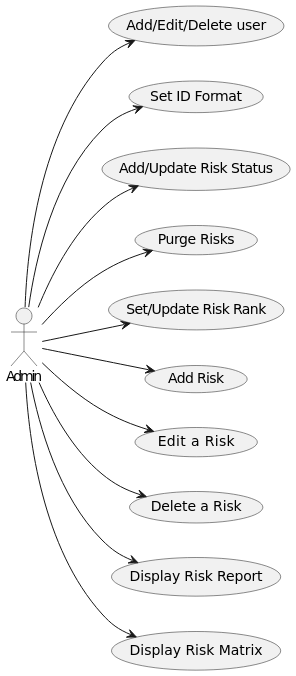
\includegraphics[width=0.4\linewidth]{AdminUserCase.jpg}
        \caption{Admin Use Case}
        \label{adminRole}
    \end{figure}
    
    A subset of activities of the admin role are managing users, as outlined below.
    
    \begin{figure} [H]
        \centering
        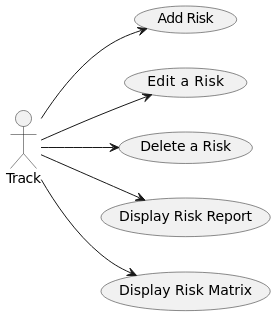
\includegraphics[width=0.5\linewidth]{TrackUserCase.jpg}
        \caption{Track Use Case}
        \label{trackRole}
    \end{figure}
    
    The track role shall have limited privileges to make necessary risk management actions, such as add risks, print risks, etc.
    
    \begin{figure} [H]
        \centering
        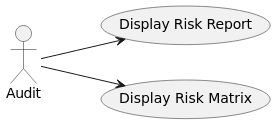
\includegraphics[width=0.5\linewidth]{AuditUserCase.jpg}
        \caption{Audit Use Case}
        \label{auditRole}
    \end{figure}
    
    The audit role shall have the most limited privileges for the purpose of only being allowed to view risks in different manners.
    
    \begin{figure} [H]
        \centering
        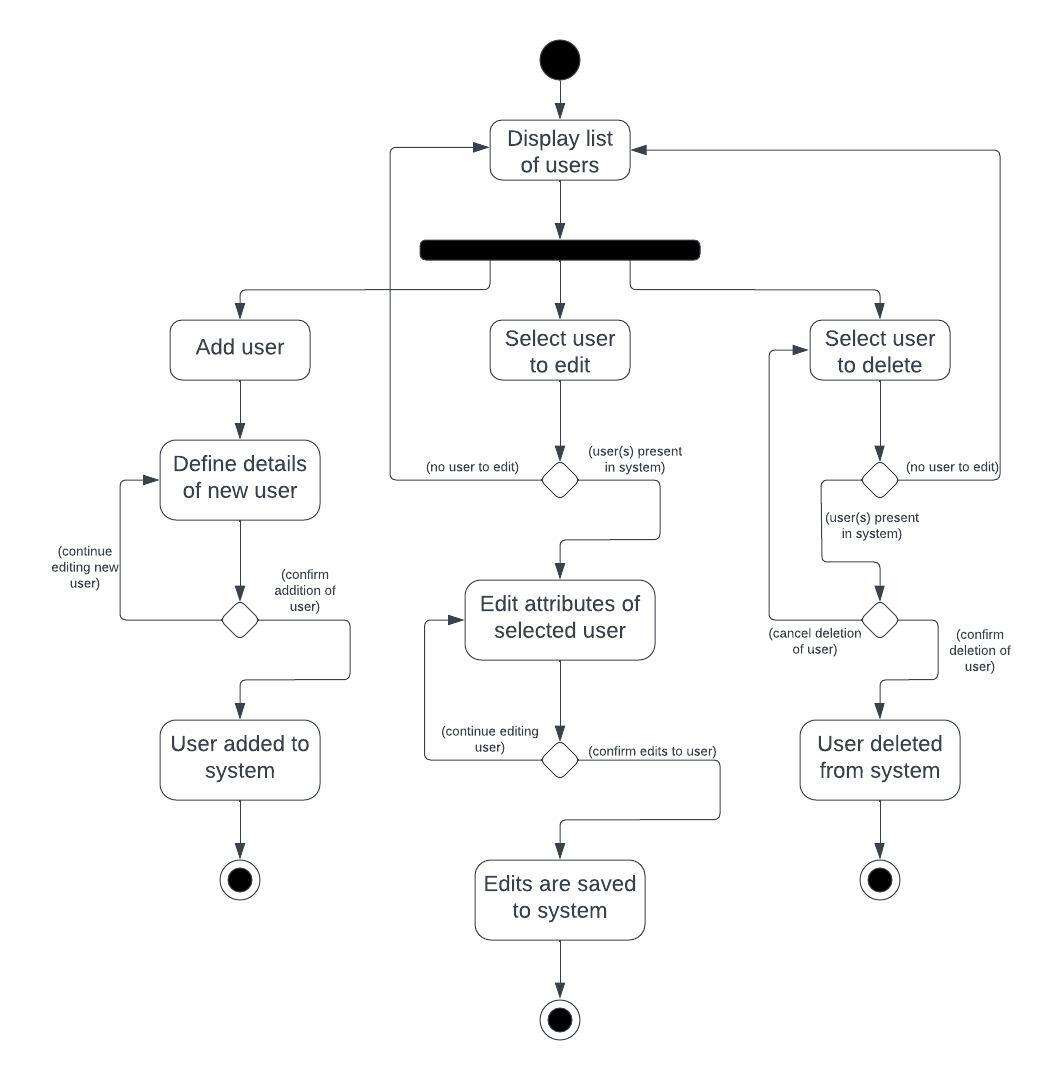
\includegraphics[width=1\linewidth]{ManageUserActivityDiagram.jpeg}
        \caption{Manage Users Activity}
        \label{manageUsers}
    \end{figure}

\section{Operating Environment}
The operating environment will be on the UNA CS Server. The CS server runs an OpenBSD OS, 64-bit, Intel/AMD compatible architecture. \\ \\
This software will be a self-contained C++ application that is accessed via http(s) in a browser (client). This will be done using the C++ STL and the Wt library, which will handle both frontend development and the server/client communication \\ \\
The software shall utilize a MySQL database for storing user and risk information. \\ \\
The system will involve many users logging in to the system to access/modify risk information based on their privilege. The software is designed for a small business that includes less than 500 people.\\ \\
The amount of disk space will depend on the amount of risks, a minimum amount would be 4GB, but may need to be scaled up. A more comfortable amount would be $16GB^+$. The disk space includes OpenBSD, MySQL, C++ STL, and Boost, along with extra space to be used to store risks.\\ \\
The RAM required is 4GB at a minimum for MySQL and the running processes, but a more comfortable amount is $8GB^+$.

\section{Design and Implementation Constraints}
Refer to Section 2.4

\chapter{NONFUNCTIONAL REQUIREMENTS}

\section{Performance Requirements}
    \begin{enumerate}
        \item This software shall respond to all user-initial actions(submissions, button clicks, or others interactions) within 1 second. Achieving this response time ensures a smooth and responsive user experience. 
        \item Optimize to handle multiple users at once this means that the system has to have the capacity to handle requests from 16 different users at once without experiencing any lag or unresponsiveness.
        \item Database Query and Stored Procedure Response Times shall be 10 milliseconds and no single query or stored procedure shall exceed 250 milliseconds in response time under typical load conditions.
    \end{enumerate}
   
\section{Safety Requirements}
    This software will ensure user safety by avoiding flashing lights that could cause injury.

\section{Security Requirements}
The software will store user credentials using a MySQL database on the CS server. User credentials will be hashed when comparing the credentials the user submits.
    

\section{Software Quality Attributes}
The product shall make use of secure coding strategies and UI standards. It shall follow the requirements set forth by stakeholders. It shall be optimized for performance where possible to reduce wait times and failures. See the SQA Plan for more details on SQA.


\chapter{STANDARDS AND REFERENCES}

\section{Applicable Standards}
% relevant standards, NIST? ISO? IEEE?
    This SRS follows applicable industry and international standards to ensure the software development process's quality and interoperability. These include:

1. IEEE 830-1998: This standard provides guidelines for SRS content and format, ensuring comprehensive documentation of software requirements.

2. ISO/IEC 12207: This international standard specifies requirements for software lifecycle processes, guiding the planning, development, testing, and maintenance of software.

3. ISO/IEC 27001: It outlines best practices for an information security management system (ISMS), ensuring the confidentiality, integrity, and availability of data.

4. ANSI/NIST-ITL 1-2011: This standard specifies data formats for the interchange of information between criminal justice organizations.


\section{References}
\subsection{Links}
\begin{itemize}
    \item{\url{https://advocacy.sba.gov/wp-content/uploads/2023/03/Frequently-Asked-Questions-About-Small-Business-March-2023-508c.pdf}}
    \item{\url{https://www.boost.org/users/history/}}
    \item{\url{https://dev.mysql.com/doc/mysql-monitor/8.0/en/system-prereqs-reference.html}}
    \item{\url{https://www.openbsd.org/faq/faq4.html\#:\~:text=OpenBSD\%20can\%20be\%20installed\%20in,more\%20disk\%20space\%20is\%20recommended.}} 
\end{itemize}


\end{document}
